\newcommand*{\TeXturedVERSION}{1.5.0} %% TeXtured 2025-08-06
%%%%%%%%%%%%%%%%%%%%%%%%%%%%%%%%%%%%%%%%%%%%%%%%%%%%%%%%%%%%%%%%%%%%%%%
%% NOTE: If you find any issues or have any suggestions, please open %%
%%       an Issue on GitHub: https://github.com/jdujava/TeXtured     %%
%%%%%%%%%%%%%%%%%%%%%%%%%%%%%%%%%%%%%%%%%%%%%%%%%%%%%%%%%%%%%%%%%%%%%%%

%% Enable built-in LaTeX support for PDF/A compliance (must be before `\documentclass`)
\DocumentMetadata{lang=en, pdfversion=1.7, pdfstandard=A-2u}
\input{preamble/pdfA-compliance/glyphtounicode}

%% NOTE: Choose the desirable page layout version (electronic vs print)
\documentclass[12pt,a4paper,twoside]{report}                      % single-side (electronic)
% \documentclass[12pt,a4paper,openright,twoside]{report}  % two-sided (for printing)
\usepackage{macros}
%% Set some toggle flags to control some of the document properties
\input{preamble/toggles}
% \FANCYfalse % disable some of the more fancy stylistic choices
%% NOTE: Comment out the following lines for the final version
\WIPtrue{}           % THIS IS A WORK-IN-PROGRESS VERSION
% \EXTRAMARGINtrue  % add extra right margin in WIP version (for notes/corrections)
% \LINKBOXESfalse   % disable reference/link boxes for faster compilations
\CENSORtrue{}         % THIS IS A CENSORED VERSION

%% Preamble - data, packages, macros, and more
\input{preamble/main}

% Add your main preamble content here

% Ensure theorem-like environments are defined
\usepackage{amsthm}
\usepackage[linesnumbered,lined,boxed,commentsnumbered]{algorithm2e}
\RestyleAlgo{ruled}
\newtheorem{remark}{Remark}
\newtheorem{result}{Result}
\newtheorem{theorem}{Theorem}
\newtheorem{lemma}{Lemma}[section]
\newtheorem{definition}{Definition}[section]
\newtheorem{example}{Example}[section]
%\newtheorem{fact}{Fact}[section]
\newtheorem{property}{Property}[section]
\newtheorem{proposition}{Proposition}[section]
\newtheorem{assumption}{Assumption}
\newtheorem{tip}{Tip}[section]
%\newtheorem{corollary}{Corollary}[section]
% \newtheorem{claim}{Claim}[section]
\newtheorem{questions}{Questions}[section]
% \newtheorem{comment}{Comment}[section]
% \newcommand{\proof}{\noindent{\bf Proof\indent}}
\newcommand{\proofover}{\hfill\vrule height8pt width6pt depth0pt\newline\noindent}

%% Only uncommented files are included (faster compilation)
%% NOTE: If no files are uncommented, all files are included
\includeonlysmart{
    frontmatter/title,
    frontmatter/approval,
    frontmatter/declaration,
    frontmatter/acknowledgements,
    frontmatter/information,
    chapters/Introduction,
    chapters/LiteratureSurvey,
    chapters/Preliminaries,
    chapters/Behavior,
    chapters/PredictiveControl,
    chapters/Summary,
}

% Ensure .aux exists (create an empty file on first run) to avoid:
%   I can't find file `thesis.aux'.
% which can stop LaTeX on the first compilation pass.
\IfFileExists{\jobname.aux}{}{%
  \newwrite\auxfile{}
  \immediate\openout\auxfile=\jobname.aux
  \immediate\write\auxfile{}%
  \immediate\closeout\auxfile{}
}

\begin{document}

\frontmatter
\pdfbookmark{Title Page}{titlepage} % add PDF outline entry
\thispagestyle{empty} % no number on the title page
\begin{center}
    \Large
    \providecommand*{\ThesisTitleFront}{\ThesisTitle}
    % {\Huge \bfseries \ThesisTitleFront \par}
    {\fontsize{22pt}{26pt}\selectfont
        \sffamily{\textbf{\ThesisTitleFront}} \par}
    \vfill
    {\fontsize{12pt}{14pt}\selectfont
        \sffamily{Submitted in the partial fulfillment of the requirements of the degree of } \par} 
    \vspace{0.5em}

    {\fontsize{14pt}{16pt}\selectfont
        \sffamily{Master of Technology} \par}
    \vspace{0.5em}
    {\fontsize{12pt}{14pt}\selectfont
        \sffamily{by} \par}
    \vspace{0.5em}
    {\fontsize{15pt}{18pt}\selectfont
        \sffamily{\ThesisAuthor} \par}
    \vspace{0.5em}
    {\fontsize{12pt}{14pt}\selectfont
        \sffamily{(Roll No: 210010061)} \par}
    \vspace{1em}
    {\fontsize{12pt}{14pt}\selectfont
        \sffamily{Supervisor:} \par}
    \vspace{0.5em}
    {\fontsize{12pt}{14pt}\selectfont
        \sffamily{\Supervisor} \par}
    \vspace{0.5em}
    {\fontsize{12pt}{14pt}\selectfont
        \sffamily{Co-Supervisors:} \par}
    \vspace{0.5em}
    {\fontsize{12pt}{14pt}\selectfont
        \sffamily{\CoSupervisor} \par}
    {\fontsize{12pt}{14pt}\selectfont
        \sffamily{\CoSupervisorAlt} \par}
    \vspace{1em}

    \begin{adjustbox}{center}
        \includegraphics[width=40mm]{iitb-logo.png}
    \end{adjustbox}

    %% if `\ThesisTitleFront` is not defined, use `\ThesisTitle`
    

    \vfill

    \sffamily\Department

    \vspace{1.1em}

    \ifFANCY\sffamily\fi
    INDIAN INSTITUTE OF TECHNOLOGY BOMBAY 
    \vspace{0.5em} \YearSubmitted \\
    \ifdef{\YearRevision}{%
        \emph{Revised version \YearRevision} \par
    }{}
    \ifWIP
        \small\ttfamily \textcolor{red}{(Draft - \today)} \par
    \fi
\end{center}

\newpage

%%% A page with a solemn declaration
\markboth{Approval Sheet}{Approval Sheet}

\centerline{\large\bfseries \sffamily Approval Sheet}

\vspace{1em}

This thesis entitled \textit{Robust Least-Squares Optimization for Data-Driven Predictive Control} by \textbf{Shreyas N. B.} is approved for the degree of \textit{Master of Technology}.

\vspace{7ex}

\renewcommand{\arraystretch}{0.8}
\arrayrulecolor{Gray70}
\begin{tabular}{cc}
\hspace{20pc} & \textbf{Examiner} \\
& \\ & \\
\hspace{20pc} & \rule{5cm}{0.4pt} \\
& \\ & \\
\hspace{20pc} & \rule{5cm}{0.4pt} \\
& \\ & \\
\hspace{20pc} & \rule{5cm}{0.4pt} \\
& \\ & \\ & \\
\hspace{20pc} & \textbf{Supervisor (s)} \\
& \\ & \\
\hspace{20pc} & \rule{5cm}{0.4pt} \\
& \\ & \\
\hspace{20pc} & \rule{5cm}{0.4pt} \\
& \\ & \\
\hspace{20pc} & \rule{5cm}{0.4pt} \\
& \\ & \\ & \\
\hspace{20pc} & \textbf{Chairperson} \\
& \\ & \\
\hspace{20pc} & \rule{5cm}{0.4pt}
\end{tabular}

\vspace{5em}
\begin{tabular}{l}
    Date: \rule{4cm}{0.4pt} \\ \\ \\
    Place: \rule{4cm}{0.4pt}
\end{tabular}

\vspace{5em}
\newpage
%%% A page with a solemn declaration
\markboth{Declaration}{Declaration}


\centerline{\large\bfseries \sffamily Declaration}

\vspace{1em}

I declare that this written submission represents my ideas in my own words and where others' ideas or words have been included, I have adequately cited and referenced the original sources.

I also declare that I have adhered to all principles of academic honesty and integrity and have not
misrepresented or fabricated or falsified any idea/data/fact/source in my submission.

I understand that any violation of the above will be cause for disciplinary action by the Institute and can also evoke penal action from the sources which have thus not been properly cited or from whom proper permission has not been taken when needed.

\textbf{I declare that I have not used any of the modern AI tools or any other similar tools for writing the thesis.}
\vspace{7ex}

\renewcommand{\arraystretch}{0.8}
\arrayrulecolor{Gray70}
\begin{tabular}{l}
\rule{6cm}{0.4pt}\\
\emph{(Signature)} \\
\\
\rule{6cm}{0.4pt}\\
\emph{(Name of the student)} \\
\\
\rule{6cm}{0.4pt}\\
\emph{(Roll No.)} \\
\\
\\
\emph{Date:} \rule{4cm}{0.4pt} \\
\end{tabular}

\vspace{5em}
\newpage
\include{frontmatter/information}
\markboth{Acknowledgments}{Acknowledgments}

\centerline{\large\bfseries \sffamily Acknowledgments}

\vspace{1em}

I would like to express my sincere gratitude to my supervisor \Supervisor , for his invaluable guidance, support, and encouragement throughout the course of this research. His insights and expertise have been instrumental in shaping the direction of this thesis.

I would also like to thank my co-supervisors \CoSupervisor \ (\emph{NTU Singapore}) and \CoSupervisorAlt \ (\emph{Microsoft, India}), for their valuable feedback and suggestions, which have greatly improved the quality of this work.

I am grateful to \textcolor{red}{Prof.~Alberto Padoan} (\emph{UBC Vancouver}) and \textcolor{red}{Prof.~Jeremy Coulson} (\emph{UW---Madison}) for generously sharing their expertise in data-driven control and behavioral theory; their insightful discussions and feedback have substantially contributed to the ideas presented in this thesis.

Finally, I would like to acknowledge the support from my Department at the Center for Systems and Control, Indian Institute of Technology Bombay, which made this research possible.


\contentsandlists{}
\mainmatter{}
\chapter{Introduction}~\label{ch:Introduction}

The objective of this thesis is to study the application of robust least-squares optimization in the context of data-driven predictive control. The fundamental idea lies in the behavioral approach to systems theory, which allows us to represent a dynamical system purely based on its observed input-output data, without requiring an explicit parametric model. This approach is particularly useful in scenarios where the underlying system dynamics are complex or unknown. 

Least-squares optimization is a classical problem which has been utilized across many domains in science and engineering over the past few centuries. The earliest documented usage of the problem can be traced back to Legendre (1805)~\cite{Legendre1805}, where it was described as an algebraic procedure for fitting linear equations to data. Legendre demonstrated the new method by analyzing the same data as Laplace for the shape of the Earth. On the other hand, Gauss (1809)~\cite{Gauss1809} went beyond Legendre and succeeded in connecting the method of least-squares with the principles of probability. The least-squares technique soon became an indispensable tool in astronomy, geodesy and laid the foundation of many core concepts in modern engineering problems.

\section{Problem Overview}

The least-squares problem is most commonly seen in the form shown below:
\begin{equation}
    \min_{x \in \R^n} \lVert A x - b \rVert_2^2,
\end{equation}
where $A \in \R^{m \times n}$ is a matrix of coefficients, $b \in \R^m$ is a vector of observations, and $x \in \R^n$ is the vector of unknowns to be determined. Thus, by minimizing the residual $\Delta b = A x - b$, it determines a solution that closely matches b in the Euclidean 2-norm. As the domain of applied statistics progressed, the total least squares problem~\cite{golub1980} was studied, which considered perturbations in both dependent and independent variables, i.e., ($\Delta A, \Delta b$). The optimal solutions may be sensitive to perturbations in the data ($A, b$). One way to mitigate this is to consider the robust least squares problem:
\begin{equation}
    \min_{x \in \R^n} \max_{A \in \mathbb{B}^{\textrm{F}}_{\rho}(\hat{A})} \lVert Ax - b \rVert_2^2,
\end{equation}
where $\mathbb{B}_{\rho}^{\mathrm{F}}(\hat{A}) = \{ A \in \R^{m \times n} : \lVert A - \hat{A} \rVert_2 \leq \rho \}$ is a ball centered around $\hat{A}$ with radius $\rho$, endowed with the Frobenius norm. 

Building on these ideas, alternative perturbation models have been explored, yielding different robust versions of the least-squares problem. For instance, El Ghaoui and Lebret (1997)~\cite{ghaoui97} considered the robust least squares problem
\begin{equation}
    \min_{x \in \R^n} \max_{[A \ b] \in \B^{\textrm{F}}_{\rho}([\hat{A} \ \hat{b}])} \lVert Ax - b \rVert_2^2.
\end{equation}
This approach is motivated by scenarios where the exact data $(A,b)$ are unknown, but belong to a family of matrices $(\hat{A} + \Delta A , \hat{b} + \Delta b)$ and the residual $[\Delta A \ \Delta b]$ lies in a norm-bounded matrix ball.

In this thesis, we introduce a robust optimization framework that accounts for the geometric nature of perturbations found in diverse instances of the problem. Specifically, we consider the optimization problem,
\begin{equation}
    \min_{x \in \R^n} \max_{\mathcal{S} \in \B^d_{\rho}(\hat{\mathcal{S}})} \lVert P_{\mathcal{S}} x - b \rVert_2^2,
\end{equation}
where $P_{\mathcal{S}}$ is the orthogonal projection onto the $k$-dimensional subspace $\mathcal{S}$ of $\R^n$, and $\mathbb{B}^d_{\rho}(\hat{\mathcal{S}})$ is a ball centered at $\hat{\mathcal{S}}$ with radius $\rho$ defined by the metric $d$ on the \textit{Grassmannian} $\Gr(k,n)$, which is  the set of all $k$-dimensional subspaces in $\R^n$ endowed with the structure of a smooth Riemannian manifold. This approach is motivated by a diverse range of applications where the linear model $A$ is a matrix representation of a subspace subject to bounded perturbations (due to uncertainty or approximations errors), quantified naturally in terms of distances between subspaces.

\section{Data-Driven Predictive Control}

The availability of large datasets coupled with unprecedented storage and computational power has recently reignited interest in direct data-driven control methods, which aim to infer optimal decisions directly from measured data (bypassing system identification). At the heart of this emerging trend lies the behavioral approach to system theory (Willems, 2007~\cite{willems2007}) and a seminal result by Willems and his collaborators \cite{willems2005}, commonly referred to as the \textit{fundamental lemma}. The lemma establishes that finite-horizon behaviors of Linear Time-Invariant (LTI) systems can be represented as images of raw data matrices. 

As a result, various data-driven modeling, estimation, filtering, and control problems can be formulated as weighted or constrained least squares problems (Markovsky and D\"orfler, 2021~\cite{markovsky2021}). Moreover, being finite-dimensional subspaces, finite-horizon LTI behaviors can be identified with points on the Grassmannian $\Gr(k, n)$ and uncertainty can be naturally quantified using Grassmannian (subspace) metrics. This approach has demonstrated its effectiveness in data-driven mode recognition and control applications and shows promise to open new avenues in adaptive control (Padoan et al., 2022~\cite{padoan2022}).

In summary, the main focus of this thesis is to explore the robust least-squares problem with subspace uncertainty and its application in data-driven predictive control via behavioral systems theory. We investigate the theoretical foundations of this approach, develop efficient algorithms for solving the robust optimization problem, and demonstrate its effectiveness through numerical simulations and real-world applications. The ultimate goal is to provide a geometric approach to robust and reliable framework for data-driven control that can handle uncertainties in the system dynamics and improve the performance of control systems in practice.
% \setcounter{chapter}{13} % "N" (14th letter, but latex first increments -> 14-1=13)
\chapter{Literature Survey} \label{ch:literature-survey}
% NOTE: since we are in the "frontmatter" part, we need to manually set headers
%       we didn't use `\chapternotnumbered`, because we want its letter in TOC,
%       and the numbering of environments to be of the form "N.1"
\markboth{Literature Survey}{Literature Survey}
\vspace{2ex}

The purpose of this chapter is to provide a survey of the existing literature related to robust least-squares, behavioral system theory, and data-driven control methods, particularly focusing on predictive control strategies. There has been significant research in this area over the past few decades, leading to various methodologies and frameworks for controlling dynamical systems using data. 

Least-squares optimization is a classical problem which has been utilized across many domains in science and engineering over the past few centuries. The earliest documented usage of the problem can be traced back to Legendre (1805)~\cite{Legendre1805}, where it was described as an algebraic procedure for fitting linear equations to data. Legendre demonstrated the new method by analyzing the same data as Laplace for the shape of the Earth. On the other hand, Gauss (1809)~\cite{Gauss1809} went beyond Legendre and succeeded in connecting the method of least-squares with the principles of probability. The least-squares technique soon became an indispensable tool in astronomy, geodesy and laid the foundation of many core concepts in modern engineering problems.

\section{Problem Overview}
\subsection{Robust Least-Squares}

The least-squares problem is most commonly seen in the form shown below:
\begin{equation}
    \min_{x \in \R^n} \lVert A x - b \rVert_2^2,
\end{equation}
where $A \in \R^{m \times n}$ is a matrix of coefficients, $b \in \R^m$ is a vector of observations, and $x \in \R^n$ is the vector of unknowns to be determined. Thus, by minimizing the residual $\Delta b = A x - b$, it determines a solution that closely matches b in the Euclidean 2-norm. As the domain of applied statistics progressed, the total least squares problem~\cite{golub1980} was studied, which considered perturbations in both dependent and independent variables, i.e., ($\Delta A, \Delta b$). The optimal solutions may be sensitive to perturbations in the data ($A, b$). One way to mitigate this is to consider the robust least squares problem:
\begin{equation}
    \min_{x \in \R^n} \max_{A \in \mathbb{B}^{\textrm{F}}_{\rho}(\hat{A})} \lVert Ax - b \rVert_2^2,
\end{equation}
where $\mathbb{B}_{\rho}^{\mathrm{F}}(\hat{A}) = \{ A \in \R^{m \times n} : \lVert A - \hat{A} \rVert_2 \leq \rho \}$ is a ball centered around $\hat{A}$ with radius $\rho$, endowed with the Frobenius norm. 

Building on these ideas, alternative perturbation models have been explored, yielding different robust versions of the least-squares problem. For instance, El Ghaoui and Lebret (1997)~\cite{ghaoui97} considered the robust least squares problem
\begin{equation}
    \min_{x \in \R^n} \max_{[A \ b] \in \B^{\textrm{F}}_{\rho}([\hat{A} \ \hat{b}])} \lVert Ax - b \rVert_2^2.
\end{equation}
This approach is motivated by scenarios where the exact data $(A,b)$ are unknown, but belong to a family of matrices $(\hat{A} + \Delta A , \hat{b} + \Delta b)$ and the residual $[\Delta A \ \Delta b]$ lies in a norm-bounded matrix ball.

In this thesis, we introduce a robust optimization framework that accounts for the geometric nature of perturbations found in diverse instances of the problem. Specifically, we consider the optimization problem,
\begin{equation}
    \min_{x \in \R^n} \max_{\mathcal{S} \in \B^d_{\rho}(\hat{\mathcal{S}})} \lVert P_{\mathcal{S}} x - b \rVert_2^2,
\end{equation}
where $P_{\mathcal{S}}$ is the orthogonal projection onto the $k$-dimensional subspace $\mathcal{S}$ of $\R^n$, and $\mathbb{B}^d_{\rho}(\hat{\mathcal{S}})$ is a ball centered at $\hat{\mathcal{S}}$ with radius $\rho$ defined by the metric $d$ on the \textit{Grassmannian} $\Gr(k,n)$, which is  the set of all $k$-dimensional subspaces in $\R^n$ endowed with the structure of a smooth Riemannian manifold. This approach is motivated by a diverse range of applications where the linear model $A$ is a matrix representation of a subspace subject to bounded perturbations (due to uncertainty or approximations errors), quantified naturally in terms of distances between subspaces.

\subsection{Data-Driven Predictive Control}

The availability of large datasets coupled with unprecedented storage and computational power has recently reignited interest in direct data-driven control methods, which aim to infer optimal decisions directly from measured data (bypassing system identification). At the heart of this emerging trend lies the behavioral approach to system theory (Willems, 2007~\cite{willems2007}) and a seminal result by Willems and his collaborators \cite{willems2005}, commonly referred to as the \textit{fundamental lemma}. The lemma establishes that finite-horizon behaviors of Linear Time-Invariant (LTI) systems can be represented as images of raw data matrices. 

The proposed idea behind data-driven predictive control via the geometric approach is posed as:
\begin{enumerate}
    \item Collect a set of input-output trajectories of the system, denoted by ${\{u_k, y_k\}}_{k=0}^{N-1}$, where $u_k \in \R^m$ and $y_k \in \R^p$ are the input and output at time step $k$, respectively. Store trajectories as $w_k = [u_k^\top \ y_k^\top]^\top \in \R^{q}$ where $q = m + p$.
    \item Construct the Hankel matrix of depth $L$ from the collected data:
    \[
        \mathcal{H}_L(w) = \begin{bmatrix}
            w_0 & w_1 & w_2 & \cdots & w_{N-L} \\
            w_1 & w_2 & w_3 & \cdots & w_{N-L+1} \\
            \vdots & \vdots & \vdots & \ddots & \vdots \\
            w_{L-1} & w_L & w_{L+1} & \cdots & w_{N-1}
        \end{bmatrix} \in \R^{qL \times (N-L+1)}.
    \]
    \item According to the fundamental lemma, if the input sequence $\{u_k\}$ is persistently exciting of order $L + n$ (where $n$ is the order of the system), then any trajectory of length $L$ can be expressed as a linear combination of the columns of $\mathcal{H}_L(w)$. In other words, the behavior $\mathfrak{B}_L$ of the system over a horizon $L$ is given by:
    \[
        \mathfrak{B}_L = \textrm{im}(\mathcal{H}_L(w)) 
    \]
    We identify $\mathfrak{B}_L$ as a $k$-dimensional subspace of $\R^{qL}$, where $k \leq qL$ is the rank of $\mathcal{H}_L(w)$. Thus, it is an element of the Grassmannian $\Gr(k, qL)$, denoted as $\mathcal{S} \equiv \mathfrak{B}_L$.
    \item At each time step $t$, solve a constrained least-squares problem to find the optimal trajectory that minimizes the cost function while satisfying the system's behavior. The optimization problem can be formulated as:
    \[
        \min_{x \in \R^{qL}} \max_{\mathcal{S} \in \B^d_{\rho}(\hat{\mathcal{S}})} \lVert P_{\mathcal{S}} x - b \rVert_2^2 , \quad \textrm{s.t.} \quad P_{\mathcal{S}}x \in \mathfrak{B}_L
    \]
   
\end{enumerate}

As a result, various data-driven modeling, estimation, filtering, and control problems can be formulated as weighted or constrained least squares problems (Markovsky and D\"orfler, 2021~\cite{markovsky2021}). Moreover, being finite-dimensional subspaces, finite-horizon LTI behaviors can be identified with points on the Grassmannian $\Gr(k, n)$ and uncertainty can be naturally quantified using Grassmannian (subspace) metrics. This approach has demonstrated its effectiveness in data-driven mode recognition and control applications (DeePC~\cite{jeremy2019}) and shows promise to open new avenues in adaptive control (Padoan et al., 2022~\cite{padoan2022}).

In summary, the main focus of this thesis is to explore the robust least-squares problem with subspace uncertainty and its application in data-driven predictive control via behavioral systems theory. We investigate the theoretical foundations of this approach, develop efficient algorithms for solving the robust optimization problem, and demonstrate its effectiveness through numerical simulations and real-world applications. The ultimate goal is to provide a geometric approach to robust and reliable framework for data-driven control that can handle uncertainties in the system dynamics and improve the performance of control systems in practice.
\chapter{Preliminaries} \label{ch:Preliminaries}

This chapter introduces mathematical concepts and notations related to optimization theory, behavioral approach to systems theory, and data-driven predictive control that will be used throughout this thesis.

\section{Geometry} \label{sec:opt}

In this section, we briefly review some fundamental concepts from Riemannian geometry and optimization on manifolds. For a more comprehensive treatment, the reader is referred to~\cite{absil,boumal2023}.

\subsection{Euclidean Spaces}
\begin{definition}[Inner Product]\label{def:euc-inner-prod}
    An inner product on a real vector space $\mathcal{E}$ is a function $\langle \cdot, \cdot \rangle : \mathcal{E} \times \mathcal{E} \to \R$ that satisfies the following properties for all $u,v,w \in \mathcal{E}$ and $a,b \in \R$:
    \begin{itemize}
        \item Symmetry: $\langle u, v \rangle = \langle v, u \rangle$,
        \item Linearity: $\langle au + bv, w \rangle = a\langle u, w \rangle + b\langle v, w \rangle$,
        \item Positive-definiteness: $\langle u, u \rangle \geq 0$ and $\langle u, u \rangle = 0 \iff u = 0$.
    \end{itemize}

\end{definition}

\begin{definition}[Euclidean Space]
    A linear space $\mathcal{E}$ equipped with an inner product $\langle \cdot, \cdot \rangle$ is called a Euclidean space. An inner product induces a norm on $\mathcal{E}$ called the Euclidean norm:
    \[
        \lVert u \rVert = \sqrt{\langle u, u \rangle}, \quad \forall u \in \mathcal{E}.
    \]
\end{definition}
The standard inner product on $\R^n$ and the associated norm are given by:
\begin{equation}\label{eq:std_inner}
    \langle u, v \rangle = u^\top v, \quad \lVert u \rVert_2 = \sqrt{u^\top u}, \quad \forall u,v \in \R^n.
\end{equation}
Similarly, the standard inner product on the space of real matrices $\R^{n \times k}$ is the Frobenius inner product, with the associated Frobenius norm:
\begin{equation}\label{eq:fro_inner}
    \langle A, B \rangle = \textrm{Tr}(A^\top B), \quad \lVert A \rVert_{\mathrm{F}} = \sqrt{\textrm{Tr}(A^\top A)}, \quad \forall A,B \in \R^{n \times k},
\end{equation}
where $\textrm{Tr}(M) = \sum_{i} M_{ii}$ denotes the trace of a matrix. We often use the following properties of the above inner product, with matrices $U, V, W, A, B$ of compatible sizes:
\begin{equation}
    \begin{split}
        \langle U, V  \rangle &= \langle U^\top, V^\top \rangle \\
        \langle A B, W \rangle &= \langle A, W B^\top \rangle = \langle B, A^\top W \rangle.
    \end{split}
\end{equation}

\begin{definition}[Differential]
    Let $U,V$ be two open sets in two Euclidean spaces $\mathcal{E}_1$ and $\mathcal{E}_2$, respectively. A map $F : U \to V$ is said to be \emph{smooth} if it is infinitely differentiable (class $\mathcal{C}^{\infty}$) on its domain. 

    Also, $F$ is said to be \emph{differentiable} at a point $x \in U$ if there exists a neighborhood $U'$of $x$ such that $F \mid_{U'}$ is smooth. Thus, if $F : U \to V$ is smooth at $x$, then its \emph{differential} at $x$, is the linear map $\textrm{D}F(x): \mathcal{E}_1 \to \mathcal{E}_2$ defined as:
    \[
        \textrm{D}F(x)[v] = \frac{d}{dt} F(x+tv) \Big|_{t = 0} =  \lim_{t \to 0} \frac{F(x + tv) - F(x)}{t}
    \]
\end{definition}

\begin{definition}[Euclidean Gradient]
    Consider a smooth function $f: \mathcal{E} \to \R$, where $\mathcal{E}$ is a linear space. The Euclidean gradient with respect to an inner product $\langle \cdot, \cdot \rangle: \mathcal{E} \times \mathcal{E} \to \R$, denoted by $\grad{f}(x)$ is a unique element of $\mathcal{E}$ such that, for all $v \in \mathcal{E}$, 
    \[
        \langle v, \grad{f}(x) \rangle = \textrm{D}f(x)[v],\quad x,v \in \mathcal{E},
    \]
    where $\textrm{D}f(x) : \mathcal{E} \to \R$ is the differential of $f$ at $x$.
\end{definition}

\begin{definition}[Euclidean Hessian]
    The Euclidean Hessian of a smooth function $f: \mathcal{E} \to \R$ is the linear map $\textrm{Hess}f(x) : \mathcal{E} \to \mathcal{E}$ defined as:
    \[
        \textrm{Hess}f(x)[v] = \textrm{D}(\grad{f})(x)[v] = \frac{d}{dt} \grad{f}(x + tv) \Big|_{t = 0}, \quad \forall x,v \in \mathcal{E}.
    \]
\end{definition}

\begin{definition}[Embedded Submanifold]
    Let $\mathcal{E}$ be a linear space of dimension $k$. A non-empty subset $\M$ of $\mathcal{E}$ is a (smooth) \emph{embedded submanifold} of $\mathcal{E}$ of dimension $n$ if either of the following conditions hold:
    \begin{enumerate}
        \item $n=k$ and $\M$ is open in $\mathcal{E}$, also called an open submanifold; or 
        \item $n=k-q$ for some $q \geq 1$ and, for each $x \in \M$, there exists an open neighborhood $U$ of $x$ in $\mathcal{E}$ and a smooth map $h : U \to \R^q$ such that:
        \begin{enumerate}[(a)]
            \item If $y$ is in $U$, then $h(y) = 0$ if and only if $y \in \M$; and
            \item \textrm{rank} $\textrm{D}h(x) = q$.
        \end{enumerate}
        Such a function $h$ is called a \emph{local defining function} for $\M$ at $x$.
    \end{enumerate}
    
\end{definition}

\begin{definition}[Tangent Space]
   Let $\M$ be a subset of $\mathcal{E}$. For all $x \in \M$, the \emph{tangent space} to $\M$ at $x$, denoted by $T_x \M$, is defined as the set of all vectors that are tangents at $x$ to smooth curves on $\M$, i.e.,
   \[
        T_x \M = \{ \gamma'(0) \mid \gamma : (-\epsilon, \epsilon) \to \M \textrm{ is a smooth curve with } \gamma(0) = x \}.
   \]
\end{definition}

\begin{definition}[Tangent Bundle]
    The \emph{tangent bundle} of a manifold $\M$ is the set of all tangent spaces over all points in $\M$:
    \[
        T\M = \{ (x,v) \mid x \in \M, v \in T_x \M \}.
    \]
\end{definition}

\subsection{Riemannian Geometry}
\begin{definition}[Differential]
    The differential of $F: \M \to \M'$ at the point $x \in \M$ is the linear map $DF(x) : T_x \M \to T_{F(x)} \M'$ defined as:
    \[
        \textrm{D}F(x)[v] = \frac{d}{dt} F(\gamma(t)) \Big|_{t = 0} = (F \circ \gamma)'(0),
    \]
    
    Let $\M$ and $\M'$ be two embedded submanifolds of two Euclidean spaces $\mathcal{E}$ and $\mathcal{E}'$, respectively. Then, the map $F : \M \to \M'$ admits a smooth extension $\bar{F} : U \to \mathcal{E}'$ defined on an open neighborhood $U$ of $\M$ in $\mathcal{E}$. Thus, for all $x \in \M$ and $v \in T_x \M$, the differential of $F$ at $x$ can be computed as:
    \[
        \textrm{D}F(x) = \textrm{D}\bar{F}(x) \mid_{T_x \M}.
    \]
\end{definition}

\begin{definition}[Riemannian Metric] \label{def:riem-metric}
    A metric $\langle \cdot, \cdot \rangle$ on $T_x \M$ is a Riemannian metric if it varies smoothly with $x$, in the sense that for all smooth vector fields $V,W$ on $\M$, the function $x \mapsto \langle V(x), W(x) \rangle_x$ is smooth.
\end{definition}

\begin{definition}[Riemannian Manifold] \label{def:riem-manifold}
    A Riemannian manifold is a smooth manifold $\M$ endowed with a \Nref*{def:riem-metric} $\langle \cdot, \cdot \rangle$.
    
\end{definition}

\begin{definition}[Riemannian Submanifold]
    An embedded submanifold $\M$ of a Euclidean space $\mathcal{E}$ is a Riemannian submanifold if it is endowed with the Riemannian metric induced by the inner product of $\mathcal{E}$, i.e., for all $x \in \M$ and $u,v \in T_x \M$,
    \[
        \langle u, v \rangle_x = \langle u, v \rangle,
    \]
    where $\langle \cdot, \cdot \rangle$ is the \Nref*{def:euc-inner-prod} on $\mathcal{E}$.
    
\end{definition}

\begin{definition}[Riemannian Gradient]
    Let $f : \mathcal{M} \to \R$ be smooth on a Riemannian manifold $\mathcal{M}$. The Riemannian gradient of $f$ is the vector field $\textrm{grad}f$ on $\mathcal{M}$ uniquely defined by the following identities:
    \[
        \forall (x,v) \in \textrm{T}\mathcal{M}, \quad \textrm{D}f(x)[v] = \langle v, \textrm{grad}f(x) \rangle_x,
    \]
    where $\textrm{D}f(x) : T_x \mathcal{M} \to \R$ is the differential of $f$ at $x$, and $\langle \cdot, \cdot \rangle_x$ is the Riemannian metric on $T_x \mathcal{M}$.
\end{definition}

\begin{definition}[Projection]
    Let $\M$ be an embedded submanifold of a Euclidean space $\mathcal{E}$ equipped with a Euclidean metric $\langle \cdot, \cdot \rangle$. The \emph{orthogonal projection} onto the tangent space $T_x \M$ at a point $x \in \M$ is the linear map $P^{\perp}_x : \mathcal{E} \to T_x \M$ which satisfies the following properties:
    \begin{enumerate}
        \item \emph{Range}: $\textrm{im}(P^{\perp}_x) = T_x \M$;
        \item \emph{Projector}: $P^{\perp}_x \circ P^{\perp}_x = P^{\perp}_x$;
        \item \emph{Orthogonal}: $\langle u - P^{\perp}_x(u), v \rangle = 0$, for all $u \in \mathcal{E}$ and $v \in T_x \M$.
    \end{enumerate}
    
\end{definition}

\begin{proposition}\label{prop:riem_grad}
    Let $\M$ be an embedded submanifold of a Euclidean space $\mathcal{E}$ equipped with a Euclidean metric $\langle \cdot, \cdot \rangle$. For a smooth function $f : \M \to \R$, the Riemannian gradient at a point $x \in \M$ is given by:
    \[
        \textrm{grad}f(x) = P^{\perp}_x(\grad{\bar{f}}(x)),
    \]
    where $\bar{f}$ is a smooth extension of $f$ to an open neighborhood of $\M$ in $\mathcal{E}$, and $\grad{\bar{f}}(x)$ is the Euclidean gradient of $\bar{f}$ at $x$.
\end{proposition}

\subsection{Grassmannians}
The Grassmannian $\Gr(k,n)$ is the set of all $k$-dimensional subspaces of $\R^n$. It can be endowed with the structure of a smooth \Nref*{def:riem-manifold} of dimension $k(n-k)$. Each point $\mathcal{S} \in \Gr(k,n)$ can be represented by an orthogonal matrix $Y \in \R^{n \times k}$ such that $Y^\top Y = I_k$.

The Grassmannian is a quotient manifold of the Stiefel manifold $\St(k,n)$, which is the set of all orthogonal $n \times k$ matrices. The equivalence class of $Y \in \St(k,n)$ is given by $[Y] = \{ Y Q \mid Q \in O(k) \}$, where $O(k)$ is the orthogonal group of $k \times k$ orthogonal matrices. Thus, $\Gr(k,n) \cong \St(k,n) / O(k)$ (refer \cite{boumal2023} for more details).

The projection operator onto the subspace $\mathcal{S}$ is given by $P_{\mathcal{S}} = Y Y^\top$ and the orthogonal complement projection is $P_{\mathcal{S}}^{\perp} = I_n - Y Y^\top$.

\begin{figure}[h]
    \centering
\begin{tikzpicture}[x={(1cm,0cm)}, y={(0.5cm,0.5cm)}, z={(0cm,1cm)}, scale=1, >=Stealth]

% Draw the subspace plane
\fill[blue!20, opacity=0.6] (0,-0.5,0) -- (3,-0.5,0) -- (3,1.5,0) -- (0,1.5,0) -- cycle;
% \draw[thick] (0,0,0) -- (3,0,0) -- (3,3,0) -- (0,3,0) -- cycle;
\node at (2.5,1,0) {$\mathcal{S}_{\hat{\mathbf{y}}}$};

% Draw coordinate axes
% \draw[->] (0,0,0) -- (4,0,0) node[below] {$x_1$};
% \draw[->] (0,0,0) -- (0,4,0) node[left] {$x_2$};
% \draw[->] (0,0,0) -- (0,0,4) node[left] {$x_3$};

% Draw vector x
\draw[->, thick, blue] (0,0,0) -- (2,1,3) node[midway, above left] {$\mathbf{x}$};

% Draw projection w = P_S x
\draw[->, thick, red] (0,0,0) -- (2,1,0) node[midway, below right ] {$\mathbf{w} = P_{\mathcal{S}_{\hat{\mathbf{y}}}}\mathbf{x}$};

% Draw perpendicular from x to w
\draw[dashed, purple] (2,1,3) -- (2,1,0) node[midway, right] {$\mathbf{x} - \mathbf{w} = P_{\mathcal{S}_{\hat{y}}}^\perp x $};

% Draw right angle indicator at w
\draw[thick, purple] (2,1,0.15) -- (1.85,1,0.12);
\draw[thick, purple] (1.85, 1,0.12) -- (1.85,1.01,-0.05);

% Origin label
% \node at (0,0,0) [below left] {$\mathbf{0}$};

\end{tikzpicture}
\caption{Depiction of the orthogonal projection of a vector onto a subspace $\mathcal{S}_{\hat{\mathbf{y}}}$.}
\end{figure}

\begin{definition}[Chordal Distance]
    The chordal distance between two subspaces $\mathcal{S}_1, \mathcal{S}_2 \in \Gr(k,n)$ is defined as:
    \[
        d_{2}(\mathcal{S}_1, \mathcal{S}_2) = \sqrt{\mathrm{Tr}\left(P_{\mathcal{S}_1}^\perp P_{\mathcal{S}_2}\right)} = \frac{1}{\sqrt{2}}\lVert P_{\mathcal{S}_1} - P_{\mathcal{S}_2} \rVert_{\mathrm{F}} = \sqrt{\sum_{i=1}^{k} \sin^2(\theta_i)},
    \]
    where $\lVert \cdot \rVert_{\mathrm{F}}$ is the Frobenius norm, and $0 \leq \theta_1 \leq \cdots \leq \theta_k \leq \pi/2$ are the principal angles between $\mathcal{S}_1$ and $\mathcal{S}_2$.
    
\end{definition}

\begin{definition}[Gap Distance]
    The gap distance between two subspaces $\mathcal{S}_1, \mathcal{S}_2 \in \Gr(k,n)$ is defined as:
    \[
        d_{\infty}(\mathcal{S}_1, \mathcal{S}_2) = \lVert P_{\mathcal{S}_1} - P_{\mathcal{S}_2} \rVert_{2} = \sin(\theta_k),
    \]
    where $\lVert \cdot \rVert_{2}$ is the spectral norm, and $\theta_k$ is the largest principal angle between $\mathcal{S}_1$ and $\mathcal{S}_2$.
    
\end{definition}

\newpage
\section{Optimization}

\begin{definition}[Convexity]
    Let $\X$ be a real vector space. Let $f: \X \to \R$ be a function, such that $x \mapsto f(x)$. Then, $f$ is convex over $\X$, for all $x \in \X$, if and only if
    \[
        f(t x_1 + (1-t)x_2) \leq t f(x_1) + (1-t)f(x_2), 
    \]
    for all $0\leq t \leq 1$, and all $x_1, x_2 \in \X$.
\end{definition}
\begin{definition}[Constrained Optimization]
    For the constrained minimization problem,
    \begin{equation}\label{eq:cons-opt}
        \min_{x \in \R^n} f(x) \quad \textrm{subject to} \quad \begin{cases}
            c_i(x) = 0, \ i \in \mathcal{E}, \\
            c_i(x) \leq 0, \ i \in \mathcal{I},
        \end{cases}
    \end{equation}
\end{definition}
where $f$ and the functions $c_i$ are all smooth, real-valued functions on a subset of $\R^n$, and $\mathcal{I}$ and $\mathcal{E}$ are two finite sets of indices. We call $f$ the \emph{objective function}, while $c_i$, $i \in \mathcal{E}$ are the equality constraints and $c_i$ , $i \in \mathcal{I}$ are the inequality constraints. We define the \emph{feasible set} $\Omega$ to be the set of points $x$ that satisfy the constraints; that is,
\[
    \Omega = \{x \mid c_i(x) = 0, i \in \mathcal{E}; c_i(x) \leq 0, i \in \mathcal{I} \},
\]
so that we rewrite the problem more compactly as,
\[
    \min_{x \in \Omega} f(x).
\]
\begin{definition}[Lagrangian function]
    The \emph{Lagrangian} function for \eqref{eq:cons-opt} is defined as:
    \[
        \mathcal{L}(x, \lambda) = f(x) + \sum_{i \in \mathcal{I} \cap \mathcal{E}} \lambda_i c_i(x) 
    \]
\end{definition}
\begin{definition}[First-Order Optimality Conditions]
    Let $x^*$ be a local solution of \eqref{eq:cons-opt}, that the functions $f$ and $c_i$ in \eqref{eq:cons-opt} are continuously differentiable. Then there exists a Lagrange multiplier $\lambda^*$, with components $\lambda_i^*, i \in \mathcal{E} \cap \mathcal{I}$, such that the following conditions are satisfied at $(x^*, \lambda^*)$,
    \begin{subequations} \label{eq:kkt}
        \begin{alignat}{4}
            \nabla_x \mathcal{L}(x^*,\lambda^*) &= 0,  \\
            c_i(x^*) &= 0, \quad i \in \mathcal{E}, \\
            c_i(x^*) &\leq 0, \quad i \in \mathcal{I}, \\
            \lambda^* & \geq 0, \quad i \in \mathcal{I}, \\
            \lambda_i^* c_i(x^*) &= 0, \quad i \in \mathcal{E} \cap \mathcal{I}. \label{eq:kkt-comp}
        \end{alignat}
    \end{subequations}
These conditions \eqref{eq:kkt} are often known as the \emph{KKT (Karush-Kuhn-Tucker) conditions}. The conditions \eqref{eq:kkt-comp} are \emph{complementarity slackness conditions}; they imply that either constraint $i$ is active or $\lambda^*_i = 0$, or possibly both.
\end{definition}

\begin{definition}[Min-Max Optimization]
In general, the min-max problems (see \cite{han2023}, \cite{han2024}) on Riemannian manifolds that we focus on, are of the kind
\[
\min_{x \in \mathcal{M}_x} \max_{y \in \mathcal{M}_y} f(x,y),
\]
where $f$ is atleast $\mathcal{C}^2$ and $\M_x,\M_y$ are the Riemannian manifolds containing $x,y$ respectively. Without loss of generality, we assume that minimization takes place first, followed by maximization (cannot be interchanged). These problems are termed \emph{min-max optimization}, whereas the candidate solution points are termed \emph{minimax points}. 

\end{definition}
\begin{definition}[Global Minimax point]
\label{def:global-minimax}
    Let $\M_x, \M_y$ be two smooth Riemannian manifolds. Consider two subsets $\X, \Y$ such that $\X \times \Y \subseteq \M_x \times \M_y$. Let $f: \X \times \Y \to \R$, be a function such that $(x,y) \mapsto f(x,y)$. The point $(x^*, y^*)$ is called a global minimax point if for any $(x,y) \in \X \times \Y$, it satisfies:
    \[
    f(x^*,y) \leq f(x^*, y^*) \leq \max_{y' \in \Y} f(x, y').
    \]
\end{definition}
\begin{definition}[Local Minimax point]
\label{def:local-minimax}
A point $(x^*, y^*)$ is a local minimax point of $f: \X \times \Y \to \R$ if there exists some $\delta_0 > 0$, and a function $h$ such that $\lim_{\delta \to 0} h(\delta) = 0 \ \forall \ \delta \in (0, \delta_0]$ and for every $(x,y) \in \X \times \Y$ satisfying $d(x,x^*) \leq \delta$ and $d(y,y^*) \leq \delta$ such that
\[
f(x^*, y) \leq f(x^*, y^*) \leq \max_{y': d(y,y') \leq h(\delta)} f(x,y').
\]
\end{definition}

\section{Systems Theory}
In this section, we briefly review some fundamental concepts in linear systems theory. Refer to~\cite{hespanha} for a comprehensive treatment.

\begin{definition}
[LTI System] \label{def:lti}
    A discrete-time linear time-invariant (LTI) system is described by the state-space equations:
    \[
        x(t+1) = A x(t) + B u(t), \quad y(t) = C x(t) + D u(t),
    \]
    where $x(t) \in \R^n$ is the state vector, $u(t) \in \R^m$ is the input vector, $y(t) \in \R^p$ is the output vector, and $A, B, C, D$ are constant matrices of appropriate dimensions.
\end{definition}

\begin{definition}
[Controllability]
    An \Nref*{def:lti} is said to be controllable if, for any initial state $x_0$ and any final state $x_f$, there exists a finite time $T$ and an input sequence $\{u(0), u(1), \ldots, u(T-1)\}$ that drives the state from $x_0$ to $x_f$ in $T$ steps.
\end{definition}

\begin{definition}
[Observability]
    An \Nref*{def:lti} is said to be observable if, for any initial state $x_0$, the output sequence $\{y(0), y(1), \ldots, y(T-1)\}$ over a finite time $T$ uniquely determines the initial state $x_0$.
\end{definition}  

\begin{definition}
[Minimal Realization]
    A realization of an \Nref*{def:lti} is said to be minimal if it has the smallest possible state dimension among all realizations that produce the same input-output behavior. A minimal realization is both controllable and observable.
\end{definition}

\begin{definition}
[Hankel Matrix]
    The Hankel matrix of an \Nref*{def:lti} is a structured matrix that captures the input-output behavior of the system. For a system with impulse response coefficients $\{h_0, h_1, h_2, \ldots\}$, the Hankel matrix $\mathcal{H}$ is defined as:
    \[
        \mathcal{H} = \begin{bmatrix}
        h_1 & h_2 & h_3 & \cdots \\
        h_2 & h_3 & h_4 & \cdots \\
        h_3 & h_4 & h_5 & \cdots \\
        \vdots & \vdots & \vdots & \ddots
        \end{bmatrix}.
    \]
\end{definition}

\begin{definition}[Kalman Rank Condition]
    An \Nref*{def:lti} is controllable if and only if the controllability matrix 
    \[
        \mathcal{C} = [B, AB, A^2B, \ldots, A^{n-1}B]
    \]
    has full row rank. Similarly, the system is observable if and only if the observability matrix
    \[
        \mathcal{O} = \begin{bmatrix}
        C \\
        CA \\
        CA^2 \\
        \vdots \\
        CA^{n-1}
        \end{bmatrix}
    \]
    has full column rank.
\end{definition}

\chapter{Behavioral Systems Theory}\label{ch:Behaviors}

The behavioral approach to systems theory, pioneered by Willems~\cite{willems2007}, offers a framework for modeling and analyzing dynamical systems based on their observed behaviors, rather than relying on explicit parametric models. In this chapter, we provide an overview of the key concepts in behavioral systems theory, including the definition of behaviors, the construction of Hankel matrices, and the fundamental lemma that underpins data-driven control methods.

\section{Behaviors}
In the behavioral framework, a dynamical system is characterized by its \emph{behavior}, which is defined as the set of all possible trajectories (input-output sequences) that the system can exhibit.

\subsection{Notation and terminology}

\subsubsection{Sets and functions}
The set of positive and non-negative integers are denoted by $\N$ and $\Z_+$, respectively. The set of real and non-negative real numbers are denoted by $\R$ and $\R_+$, respectively.  
For ${T\in\N}$, the set of integers $\{1, 2, \dots , T\}$ is denoted by $\mathbf{T}$.  A map $f$ from $X$ to $Y$ is denoted by ${f:X \to Y}$; $(Y)^{X}$ denotes the set of all such maps. The \textit{restriction} of ${f:X \to Y}$ to a set ${X^{\prime}}$, with ${X^{\prime} \cap X \neq \emptyset}$, is denoted by $f|_{X^{\prime}}$ and is defined by $f|_{X^{\prime}}(x)$ for ${x \in X^{\prime}}$; if ${\mathcal{F} \subseteq (Y)^{X}}$, then $\mathcal{F}|_{X^{\prime}}$ is defined as ${\{ f|_{X^{\prime}} \, : \, f \in \mathcal{F}\}}$.

\subsubsection{Linear algebra}
The transpose, image, and kernel of a matrix ${M\in\R^{m\times n}}$ are denoted by $M^{\top}$, $\Image\, M$, and $\Ker M$, respectively. The $m \times p$ zero matrix is denoted by $0_{m \times p}$ and the $m \times p$ matrix with ones on the main diagonal and zeros elsewhere is denoted by $I_{m \times p}$. For $m = p$, we use $0_p$ and $I_p$, and subscripts are omitted when dimensions are clear from context. The Kronecker product of the matrices $M \in \R^{m \times n}$ and $N \in \R^{p \times q}$ is denoted by $M \otimes N$. 


\subsection{Sequences, shift operator, Hankel matrices}

 A \textit{sequence} is a function ${w: S \to \R^q}$, where ${S \subseteq \N}$; the sequence is \textit{finite} if $S$ has finite cardinality, and \textit{infinite} otherwise. An infinite sequence ${w}$ is also denoted by $\{w_k\}_{k\in\N}$. We use the terms \textit{sequence}, \textit{time series}, and \textit{trajectory} interchangeably.  By a convenient abuse of notation, a finite sequence ${w\in(\R^q)}^\mathbf{T}$ is often identified with the corresponding column vector ${w=\col(w(1),\ldots,w(T))\in\R^{qT}}.$

The \textit{shift operator} ${\sigma : {(\R^q)}^\N \to {(\R^q)}^\N}$ is defined as
 \begin{equation}
    \sigma w (t)= w(t+1).
 \end{equation}

 By convention, the shift operator acts on all elements of a set ${\mathcal{W} \subseteq {(\R^q)}^\N}$, that is, $\sigma \mathcal{W}  =\{\sigma w\,:\, w\in\mathcal{W} \}$.

The \textit{Hankel matrix} of depth ${L\in\mathbf{T}}$ associated with the sequence ${w\in {(\R^q)}^\mathbf{T}}$ is defined as 
 \begin{equation} \label{eq:Hankel} 
 \mathcal{H}_{L}(w) =
 \begin{bmatrix}
    w(1) & w(2) & w(3) & \cdots & w(T-L+1) \\
    w(2) & w(3) & w(4) & \cdots & w(T-L+2) \\
    \vdots & \vdots & \vdots & \ddots & \vdots \\
    w(L) & w(L+1) & w(L+2) & \cdots & w(T)
 \end{bmatrix}
 \end{equation}

 \subsubsection{Systems}
 In behavioral systems theory~\cite{willemspolderman1998}, a \textit{system} is a triple $\Sigma=(\T,\W,\Be),$ where $\T$ is the \textit{time set}, $\W$ is the \textit{signal set}, and $\Be \subseteq (\W)^{\T}$ is the \textit{behavior} of the system. Throughout this work, we exclusively focus on \textit{discrete-time} systems, with ${\T = \N}$ and ${\W = \R^q}$. We adapt definitions accordingly, emphasizing this assumption when necessary. By a convenient abuse of notation, we also identify a system $\Sigma$ with the corresponding behavior $\Be$.

 \subsubsection{LTI systems}
 A system $\Be$ is \textit{linear} if $\Be$ is a linear subspace, \textit{time-invariant} if $\Be$ is shift-invariant, \textit{i.e.}, ${\sigma(\Be) \subseteq \Be}$, and \textit{complete} if ${w\in\Be}$ if and only ${w|_{[t_0,t_1]} \in \Be|_{[t_0,t_1]}}$ for every ${-\infty < t_0 \le t_1 < \infty}$. Completeness of a discrete-time linear system $\Be$ is equivalent  to $\Be$ being closed in the topology of pointwise convergence~\cite[Proposition 4]{willems1986}. The set of all (discrete-time) complete LTI systems is denoted by $\mathcal{L}^q$.  By a convenient abuse of notation, we often write $\Be \in \mathcal{L}^{q}$.


 \subsubsection{Kernel representations}
 Every LTI system ${\Be \in \mathcal{L}^{q}}$ admits a \textit{kernel representation} of the form
 \begin{equation}
 \Be = \Ker R(\sigma) ,
 \end{equation}
 where  $R(\sigma)$ is the operator defined by the polynomial matrix 
\[
R(z) = R_1 + R_2 z + \cdots + R_{d}z^{d-1},
\]
 with $R_i\in\R^{g\times q}$ for $i\in\text{\boldmath$d$\unboldmath},$ and 
 \[
   \Ker R(\sigma) = \{w\in{(\R^q)}^\N \,:\, R(\sigma)w = 0\}.
 \]
 Without loss of generality, one may assume that  $\Ker R(\sigma)$  is a \emph{minimal}  kernel representation of $\B$,  \textit{i.e.},  $R(\sigma)$ has full row rank~\cite{willems1989}.


 \subsubsection{Partitions}
 Given a permutation matrix ${\Pi\in\R^{q\times q}}$ and an integer $0 < m < q$, the map defined by the equation
 \begin{equation} \label{eq:partition} 
 (u,y) = \Pi w 
 \end{equation}
 induces a \textit{partition} of each ${w\in\R^q}$ into the variables ${u\in\R^m}$ and ${y\in\R^{q-m}}$.  For LTI systems, we can also simply identify trajectories as 
 \begin{equation} \label{eq:partition_lti}
   w = \begin{bmatrix}
      u \\
      y
   \end{bmatrix}
 \end{equation}
 We write $w \sim (u,y)$ if~\eqref{eq:partition} holds for some  permutation matrix ${\Pi\in\R^{q\times q}}$ and integer ${0 < m < q}$.  
 Any partition~\eqref{eq:partition} induces natural  projections  ${ \pi_u:  w \mapsto u}$ and ${ \pi_y:  w \mapsto y}$. We call~\eqref{eq:partition} a \textit{partition of ${\Be\in\mathcal{L}^{q}}$} if~\eqref{eq:partition} holds for all ${w\in\Be}$; the partition~\eqref{eq:partition} is an \textit{input-output partition} if $u$ is an \textit{input} and $y$ is an \textit{output} (see~\cite[p.568]{willems1986} for definitions).

 \subsubsection{Integer invariants}
 The structure of an LTI  system ${\Be \in\mathcal{L}^q}$ is characterized by a set of \textit{integer invariants}~\cite{willems1986}, defined as
 \begin{itemize}
 \item the \textit{number of inputs} ${m(\Be) = q-\text{row dim} R(\sigma)}$,  
 \item the \textit{number of outputs} ${p(\Be) = \text{row dim} R(\sigma)}$,  
 \item the \textit{lag} ${\ell(\Be) = \max_{i \in\mathbf{p}}\{\deg\text{row}_i R(\sigma) \}}$, and
 \item the \textit{order} ${n(\Be)=\sum_{i \in\mathbf{p}} \deg\text{row}_i R(\sigma) }$, % ${n=\ell_1+ \ldots+ \ell_p}$,
 \end{itemize}
 where   
 $\Ker R(\sigma)$  is a minimal  kernel representation of $\Be$, while   
 ${\text{row dim}R}$ and ${\deg\text{row}_i R}$ are the number of rows and the degree of the $i$-th row of $R(z)$, respectively. The integer invariants are intrinsic properties of a system, as they do not depend on its representation~\cite{willems1986}. Thus, we omit the dependence on the particular behavior if clear from context.


 \subsubsection{Latent variables} 
 A \textit{system with latent variables} is a tuple $\Sigma = (\N, \R^q, \R^\kappa, \Be_{\textup{full}})$, where $\N$ is the \textit{time set}, $\R^q$ is the set of \textit{manifest variables}, $\R^\kappa$ is the set of \textit{latent variables}, and $\Be_{\textup{full}} \subseteq (\R^q \times \R^\kappa)^{\N}$ is the \textit{full behavior}, respectively. The \textit{manifest behavior} of the system is defined as
 \begin{equation}
 \Be_{\textup{man}} = \{ w \in (\R^q)^\N \mid \exists \, \eta\in(\R^\kappa)^\N \text{ s.\,t. } (w, \eta) \in \Be_{\textup{full}} \},
 \end{equation}
 where $w$ is the \textit{manifest variable} and $\eta$ is the \textit{latent variable}. Manifest variables are \textit{external} and directly observable (e.g., inputs and outputs); latent variables are \textit{internal} (e.g., state and interconnection variables) and usually play an auxiliary~role.


 \subsubsection{State-space representations}
 Every finite-dimensional LTI dynamic system ${\B \in \mathcal{L}^{q}}$ can be described by the equations
 \begin{equation} \label{eq:state-space}
 \sigma x = Ax + Bu, \quad y=Cx+Du,
 \end{equation}
 and admits a (\textit{minimal}) \textit{input/state/output representation} 
 \begin{equation} \label{eq:partition-ISO} 
 \!  \! \Be \!  = \!
 \left\{  (u,y) \sim w \in (\R^{q})^\N \,:\, \exists \,x\in(\R^n)^{\N} \, \textup{s.t.}~\eqref{eq:state-space}~\text{holds}
 \right\},
 \end{equation}
 where
 \[
    \begin{bmatrix}
    A & B \\
    C & D
    \end{bmatrix} \in \R^{(n+p)\times (n+m)}
 \]
   and  $m$, $n$, and $p$ are the number of inputs, the order, and the number of outputs of $\Be$, respectively. State-space representations define systems where the latent variable is the state $x$.

\subsubsection{Data-driven representations}
 
Data-driven representations connect data directly to system behavior using data matrices. The restricted behavior of a finite-dimensional,  discrete-time, LTI system is a subspace, whose dimension is determined only by the integer invariants and time horizon.


 \begin{lemma}\cite[Lemma 2.1]{dorfler2022} \label{lemma:subspace}
 Let ${\Be \in \mathcal{L}^{q}}$ and ${L\in\N}$. The restricted behavior $\Be|_{[1,L]}$ is a subspace of $(\R^{q})^{\mathbf{L}}$ and ${\dim \Be|_{[1,L]}  =  m(\Be) L+ n(\Be)}$ for all ${L>\ell(\Be)}$. 
 \end{lemma}

As a direct consequence of Lemma~\ref{lemma:subspace}, the restricted behavior of a finite-dimensional, discrete-time,  LTI system can be represented as the image of a raw data matrix. Next, we summarize a version of this principle known as the \textit{fundamental lemma}~\cite{willems2005}.

\begin{lemma}~\cite[Corollary 19]{markovsky2020} \label{lemma:fundamental_generalized}
 Let ${\Be \in \mathcal{L}^{q}}$ and ${w \in \Be|_{[1,T]}}$. Fix $L\in\mathbf{T}$, with ${L > \ell(\Be)}$. Then  $\Be|_{[1,L]} = \Image  \mathcal{H}_L(w)$  if and only if
 \begin{equation}  \label{eq:generalized_persistency_of_excitation} 
 \rank  \mathcal{H}_L(w)   =  m(\Be)L+ n(\Be).
 \end{equation}
 \end{lemma}

\noindent
The rank condition~\eqref{eq:generalized_persistency_of_excitation} is referred to as the  \emph{generalized persistency of excitation} condition~\cite{markovsky2020}. Thus, we call a trajectory ${w \in \Be|_{[1,T]}}$ of a system ${\Be \in \mathcal{L}^{q}}$ \emph{generalized persistently exciting (GPE) of order $L$} if~\eqref{eq:generalized_persistency_of_excitation} holds. Different variations of this principle can be formulated under a range of assumptions, see, \textit{e.g.}, the recent survey~\cite{markovsky2021} for an overview and~\cite{padoan2022} for some extensions to broader classes of systems.

\newpage
\section{System Identification}

System identification in the behavioral framework involves constructing a behavior $\Be$ that accurately captures the dynamics of a system based on observed data. 

Using the fundamental lemma (Lemma~\ref{lemma:fundamental_generalized}), one can identify the behavior of a finite-dimensional, discrete-time, LTI system from a set of GPE trajectories. Specifically, given a set of trajectories ${\{w_i\}}_{i=1}^{T_d}$ that are GPE of order $L$, the restricted-behavior can be reconstructed as
\begin{equation}
   \Image \mathcal{H}_L(w) = \Be_{[1,L]}
\end{equation} 

\subsection{Effect of noise}
In practical scenarios, data is often corrupted by noise, which can affect the accuracy of (behavioral) system identification. The rank of the Hankel matrix may be inflated due to noise, masking the system's actual order. To mitigate this, techniques such as singular value decomposition (SVD) can be employed to approximate the Hankel matrix and extract the dominant dynamics.

The singular values of the Hankel matrix can provide insights into the underlying system order, allowing for a more robust identification process in the presence of noise. An analysis of the magnitude of singular values for noisy data and ideal data is shown in Figure~\ref{fig:svd_noise}, which was performed for a simple SISO system (double integrator) with $10\%$ additive Gaussian noise. It can be observed that the presence of noise inflates the singular values, masking the true system order. The noise floor, indicated by the dashed line, is where the singular values suddenly drop off, suggesting a cutoff for identifying the system order in the ideal case.

\begin{figure}[h]
      \centering
      \includegraphics[width=\textwidth]{figures/noise_floor.png}
      \caption{Singular values of Hankel matrices constructed from ideal data (blue) and noisy data (red). The noise floor is shown by the dashed line.}
      \label{fig:svd_noise}
\end{figure}

\subsection{Grassmannians and Behaviors}
Behaviors can be viewed as points on a Grassmannian manifold, which is the space of all $k$-dimensional subspaces of an $n$-dimensional vector space. This perspective allows for the application of geometric methods in system identification and analysis.

Given restricted behavior $\Be|_{[1,L]}$ of dimension $k = m(\Be)L + n(\Be)$, we can associate it with a point on the Grassmannian manifold $\Gr(k, qL)$.

Denote $r_H = \rank \mathcal{H}_L(w)$ for trajectories ${\{w_i\}}_1^{T_d}$. Depending on the noise level, $r_H$ satisfies the following:
\begin{equation}
  k \leq r_H \leq n,
\end{equation}
where $n = qL, k = m(\Be)L + n(\Be)$. Still, only the first $k$ singular vectors of $\mathcal{H}_L(w)$ correspond to the behavior $\Be$. Thus, the behavior can be identified with a point on the Grassmannian manifold $\Gr(k, n)$. To obtain an orthonormal basis for the behavior, we can perform an SVD on $\mathcal{H}_L(w)$ and extract the first $k$ left singular vectors. This basis spans the same subspace as $\Be|_{[1,L]}$, providing a representation of the behavior in the presence of noise. Thus,
\begin{equation}
   \mathcal{H}_L(w) = U \Sigma V^\top,
\end{equation}
where $U \in \R^{n \times r_H}$, $\Sigma \in \R^{r_H \times r_H}$, and $V \in \R^{(T_d-L+1) \times r_H}$. The first $k$ columns of $U$, is equivalently denoted by $\hat{Y}$ such that
\begin{equation}
   \hat{Y} \equiv U_{[1:k]},
\end{equation}
where $\hat{Y} \in \R^{n \times k}$ and $\hat{Y}^\top \hat{Y} = \I_k$. The subspace spanned by the columns of $\hat{Y}$ corresponds to the behavior $\Be|_{[1,L]}$, is also identified by $\hat{S} \in \Gr(k,n)$.

\subsubsection{Summary}
\begin{figure}[h]
   \centering
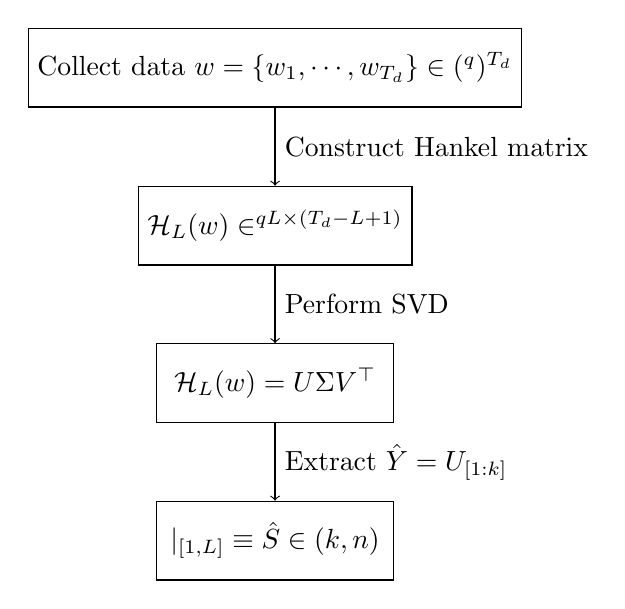
\begin{tikzpicture}[scale=0.6]
   \node (data) [draw, rectangle, minimum width=3cm, minimum height=1cm] {Collect data $w = \{w_1, \cdots, w_{T_d}\} \in {(\R^{q})^{T_d}}$};
   \node (hankel) [draw, rectangle, minimum width=3cm, minimum height=1cm, below=1.5cm] { $\mathcal{H}_L(w) \in \R^{qL \times (T_d-L+1)}$};
   \node (svd) [draw, rectangle, minimum width=3cm, minimum height=1cm, below=3.5cm] {$\mathcal{H}_L(w) = U \Sigma V^\top$};
   \node (grassmannian) [draw, rectangle, minimum width=3cm, minimum height=1cm, below=5.5cm] {$\Be|_{[1,L]} \equiv \hat{S} \in \Gr(k,n)$};
   \draw[->] (data) -- (hankel) node[midway, right] {Construct Hankel matrix};
   \draw[->] (hankel) -- (svd) node[midway, right] {Perform SVD};
   \draw[->] (svd) -- (grassmannian) node[midway, right] {Extract $\hat{Y} = U_{[1:k]}$};
\end{tikzpicture}
\end{figure}





\chapter{Data-Driven Control}\label{ch:DDC}



\backmatter{}
%% NOTE: uncomment following line if you use parts in your document
% \addtocontents{toc}{\vspace{2ex}}  % Add extra space after the last part in TOC

\chapternotnumbered{Summary and Future Work}

\label{ch:Summary}
\vspace{2ex}
This thesis has explored the application of robust least-squares optimization in the context of data-driven predictive control, leveraging the behavioral approach to systems theory. By representing dynamical systems based on observed input-output data, we have developed a geometric framework that effectively handles uncertainties in system dynamics.

The key contributions of this work include:
\begin{enumerate}
    \item Development of a robust least-squares optimization framework that accounts for subspace uncertainty, enabling more reliable control strategies in the presence of data perturbations.
    \item Integration of the behavioral approach to system theory, allowing for a flexible representation of dynamical systems without explicit parametric models.
    \item Formulation of data-driven predictive control problems as constrained least-squares problems, facilitating the design of control strategies directly from observed data.
    \item Demonstration of the effectiveness of the proposed framework through numerical simulations.
\end{enumerate}

Future research directions include:
\begin{itemize}
    \item Extension of the robust least-squares framework to accommodate linear time-varying (LTV) systems and nonlinear systems.
    \item System-theoretic interpretation of the worst-case subspace $Y^\star$ in the context of robust or $H_\infty$ control.
    \item Enhancing the computational efficiency of the proposed algorithms using advanced optimization techniques like adaptive time-stepping, etc.
    \item Experimental validation of the proposed framework on real-world systems to assess its practical applicability and performance.
\end{itemize}

% \appendix
% \include{chapters/Appendix}

\references{}

\end{document}
